\section{Agenda}

\begin{frame}
    \begin{itemize}
            \item item 1
            \item $\ldots$
            \begin{itemize}
                \item test
                \item $\ldots$
            \end{itemize}
        \end{itemize}
\end{frame}

\section{Next Section}

\begin{frame}
    \frametitle{Benchmarking Setup}
    \begin{figure}
    \noindent\hspace{1mm}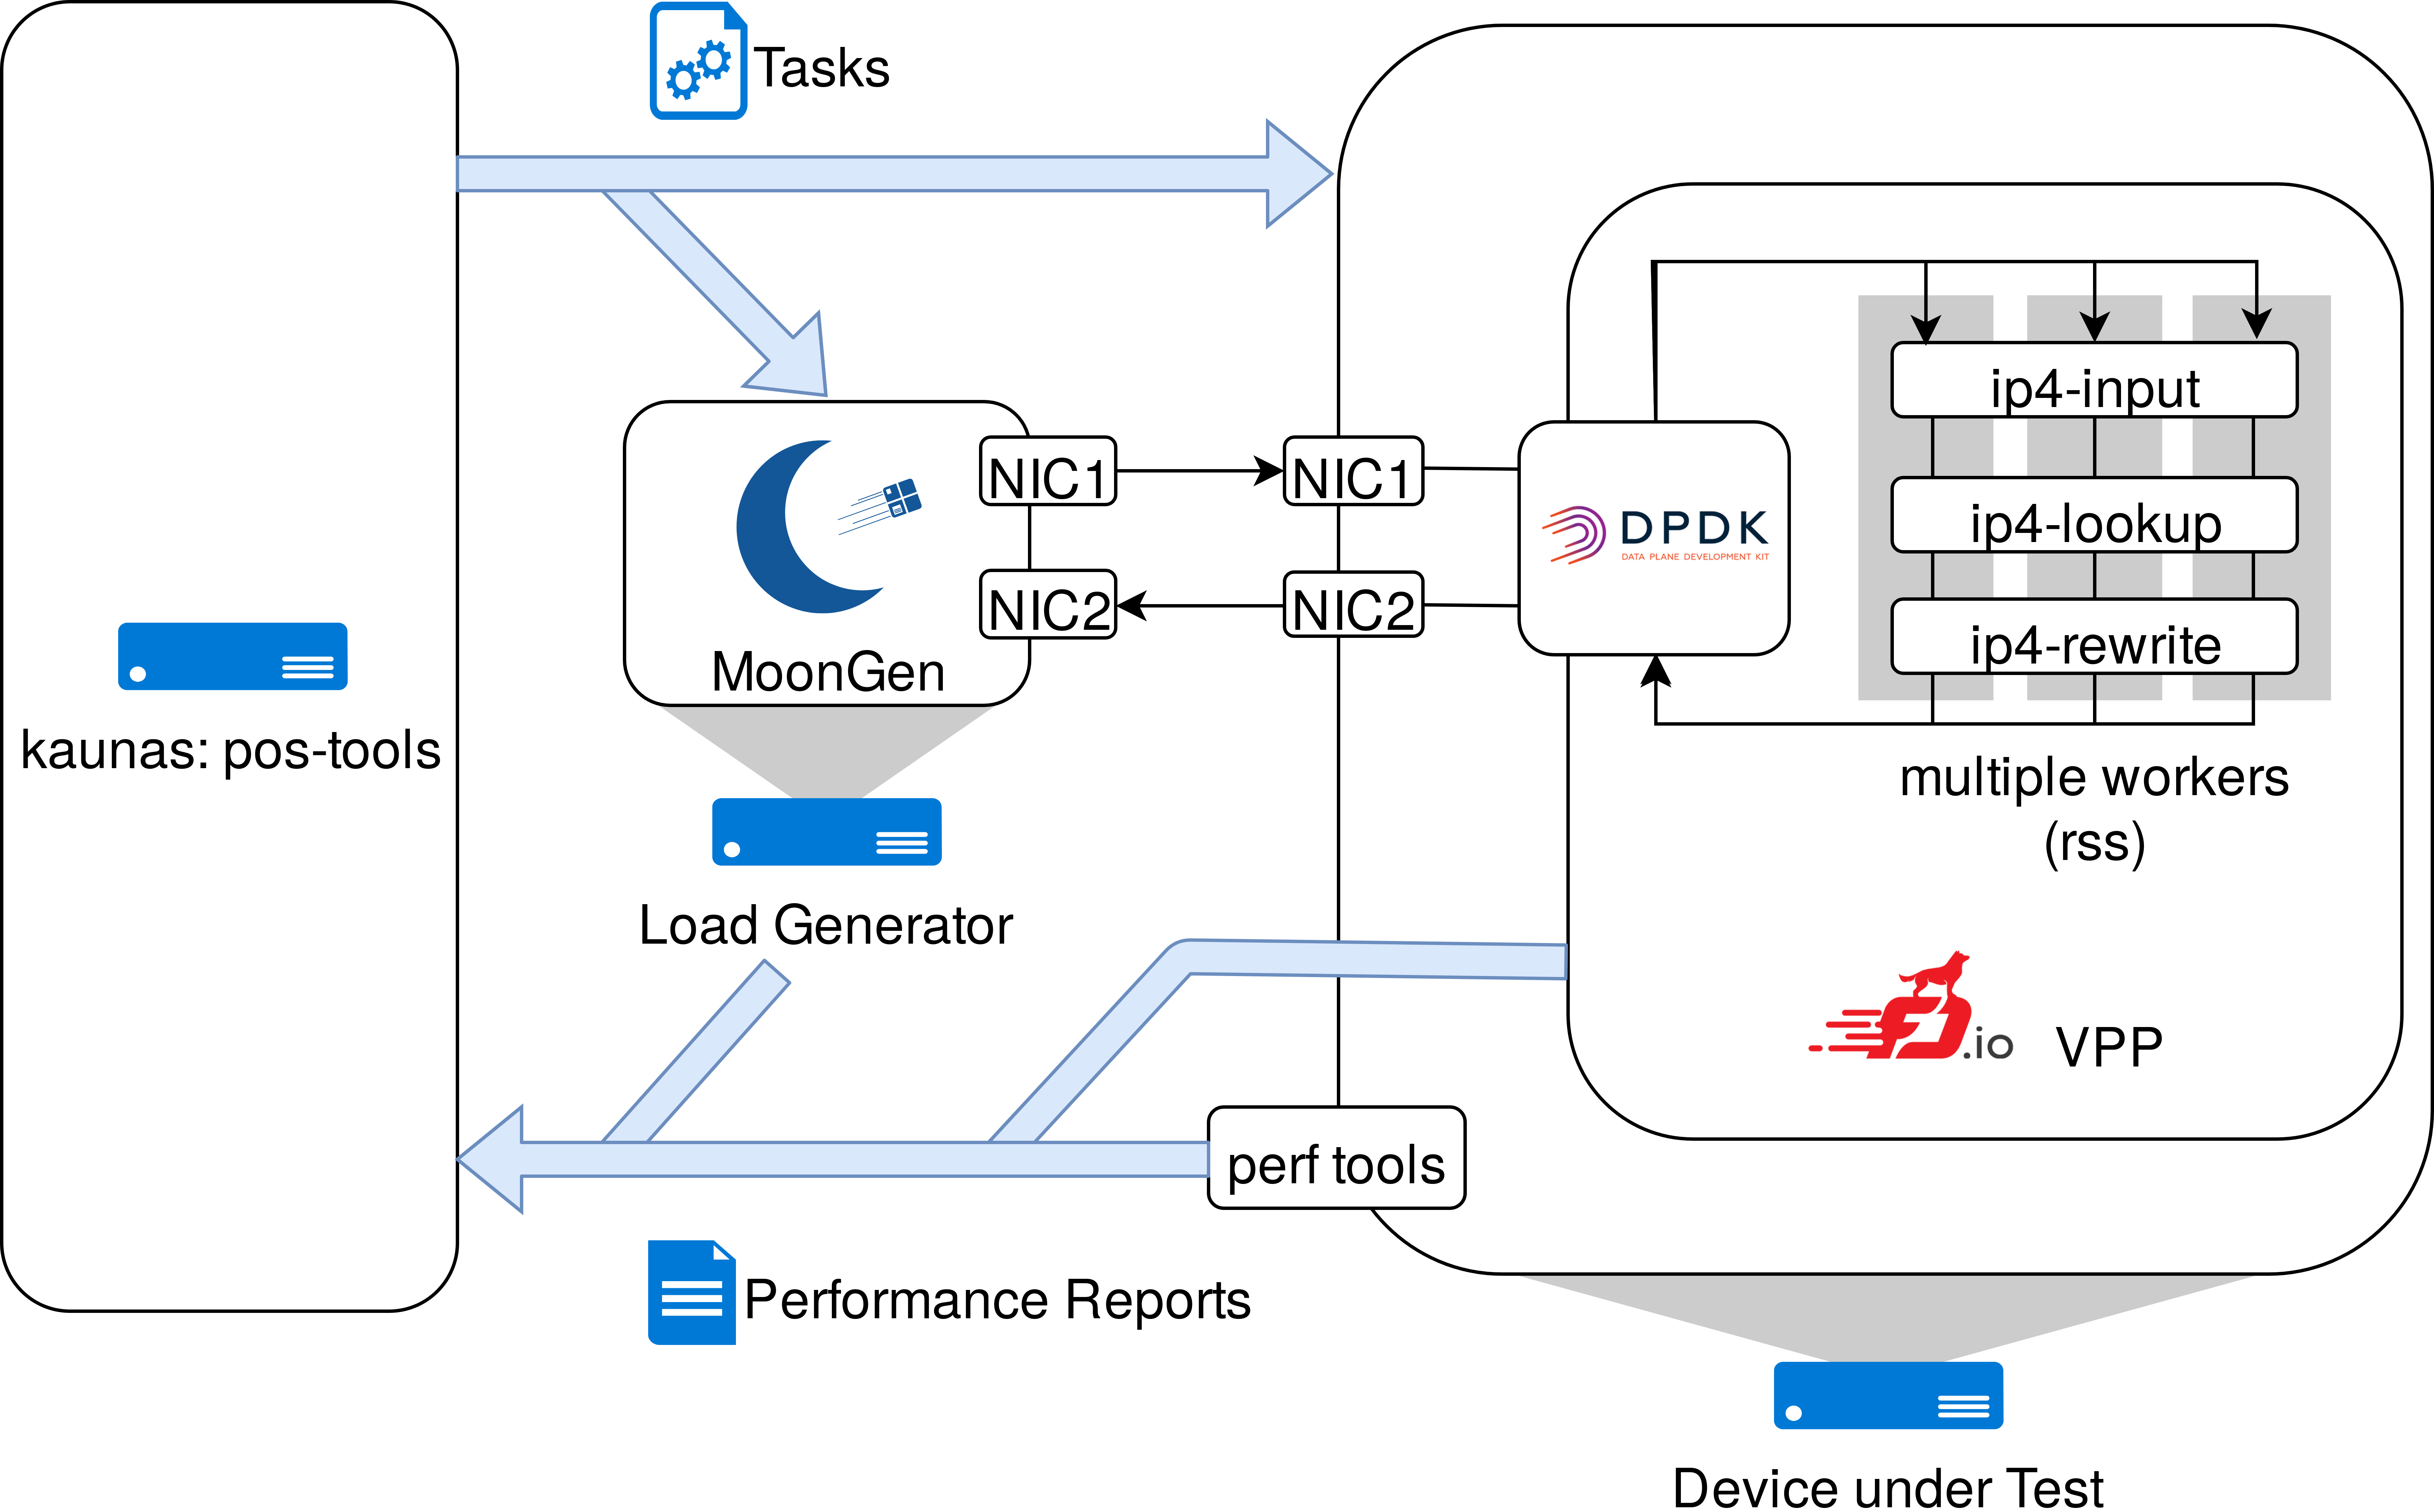
\includegraphics[width=\linewidth]{pics/topology.png}
    %\caption{Experiment setup for testing VPP with "kaunas" management server, LoadGen and DUT}
    \label{setup}
    \end{figure}
\end{frame}


\begin{frame}
    \frametitle{Packet Processing Graph}
    \begin{figure}
    \noindent\hspace{1mm}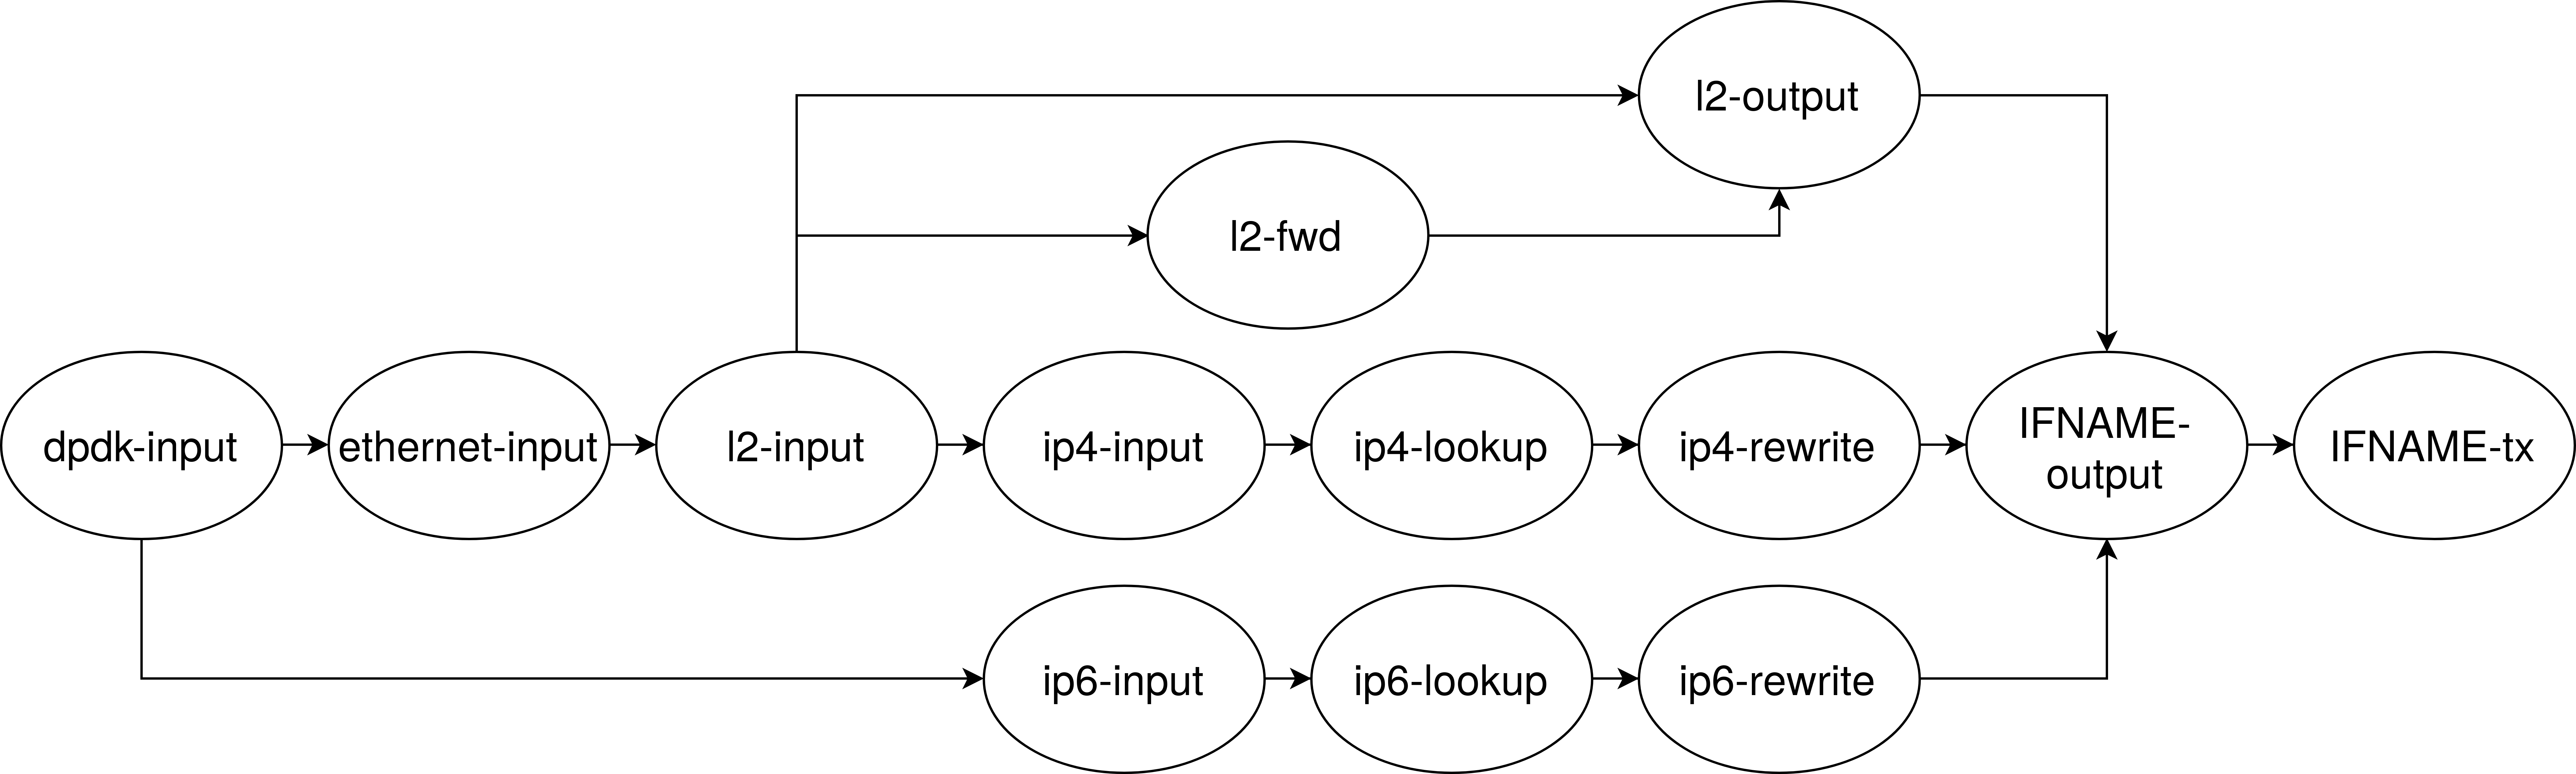
\includegraphics[width=\linewidth]{pics/vpp-nodes-horizontal.png}
    \caption{VPP packet processing graph for xconnect, bridging, IPv4 routing and IPv6 routing. Other paths are left out. }
    \label{nodegraph}
    \end{figure}
\end{frame}

\section{Tests Conducted}

\begin{frame}
    \frametitle{Scenarios}
    Scenarios:
    
\end{frame}

\begin{frame}
    \frametitle{Parameters}
\end{frame}

\section{Conclusion}


\begin{frame}
    \frametitle{Comparison}
    % TODO graphical visualization
    \begin{table}
        \begin{tabular}[]{ l r r r }
            Implementation   & FIB sizes & Mpps     & Relative \\ 
            \midrule
            MoonRoute        & 1         & 14.6     & 100\% \\
            MoonRoute        & $2^{20}$  & 14.2     & 97\% \\
            MoonRoute        & $2^{24}$  & 11.6     & 79\% \\
            VPP v18.10       & 1         & 11.6     & 79\% \\
            FastClick DPDK   & 1         & 10.4     & 72\% \\
            FastClick DPDK   & $2^{20}$  & 10.4     & 72\% \\
            VPP v16.09       & 1         & 9.7      & 71\% \\
            VPP v16.09       & 255k      & 9.2      & 63\% \\
            VPP v16.09       & $2^{20}$  & 8.5      & 58\% \\
            VPP v18.10       & 255k      & 7.2      & 50\% \\
            VPP v16.09       & $2^{23}$  & 6.5      & 45\% \\
            Click DPDK       & 1         & 4.3      & 29\% \\
            Click DPDK       & $2^{20}$  & 4.2      & 28\% \\
            Linux 3.7        & 1         & 1.5      & 11\% \\

            \midrule
        \end{tabular}
        \caption{Comparison of maximum IPv4 forwarding throughput with a single worker on the Xeon E3-1230 system. Non-VPP results are from \cite{chair:architecture} and are conducted on the same system. }
        \label{table:comparison}
    \end{table}
\end{frame}



\section{Questions?}

\begin{frame}
    \frametitle{Example frame}
    \begin{itemize}
        \item item 1
        \item $\ldots$
        \begin{itemize}
            \item test
            \item $\ldots$
        \end{itemize}
    \end{itemize}
    Citation \cite{rfc959}

    \paragraph{Math mode should be fully functional:}
    $$
    \hat s
    \overline s
    \mathcal S
    \mathbit S
    \mathbit \Lambda
    \sum
    \pd{\xi}
    \pr{X=0}
    \mathbit 1
    $$
\end{frame}

\begin{frame}
    \frametitle{Figures}
    \begin{figure}
        \centering
        \includegraphics[width=.5\textwidth]{figures/example}
        \caption{Figure caption}
        \label{Maizaso0}
    \end{figure}
    Figure~\ref{Maizaso0} shows a small network.
\end{frame}

\begin{frame}
    \frametitle{Figures}
    \begin{table}
        \begin{tabular}{rccc}
            \toprule
            & Competitor 1 & Competitor 2 & we\\
            \midrule
            Feature A & \no & \maybe & \yes\\
            Feature B & \no & \maybe & \yes\\
            Feature C & \no & \maybe & \yes\\
            Feature D & \no & \maybe & \yes\\
            \bottomrule
        \end{tabular}
    \end{table}
\end{frame}

